%----------------------------------------------------------------------------------------
%	CHAPTER 2
%----------------------------------------------------------------------------------------
\chapterimage{band1.png}

\chapter{Discovering what to do...}

\section{First ideas}\index{First ideas}
So, now here you have your first astronomy picture, \footnote{For example purposes the image selected is a picture of M83 through a Wide H-alpha and [N II] filter. } what do you see?, it is a monochrome image, with different levels of brightness, slightly big (8500 x 5000), it looks like a lot of stars making a spiral.
\begin{figure}[h]
    \centering
    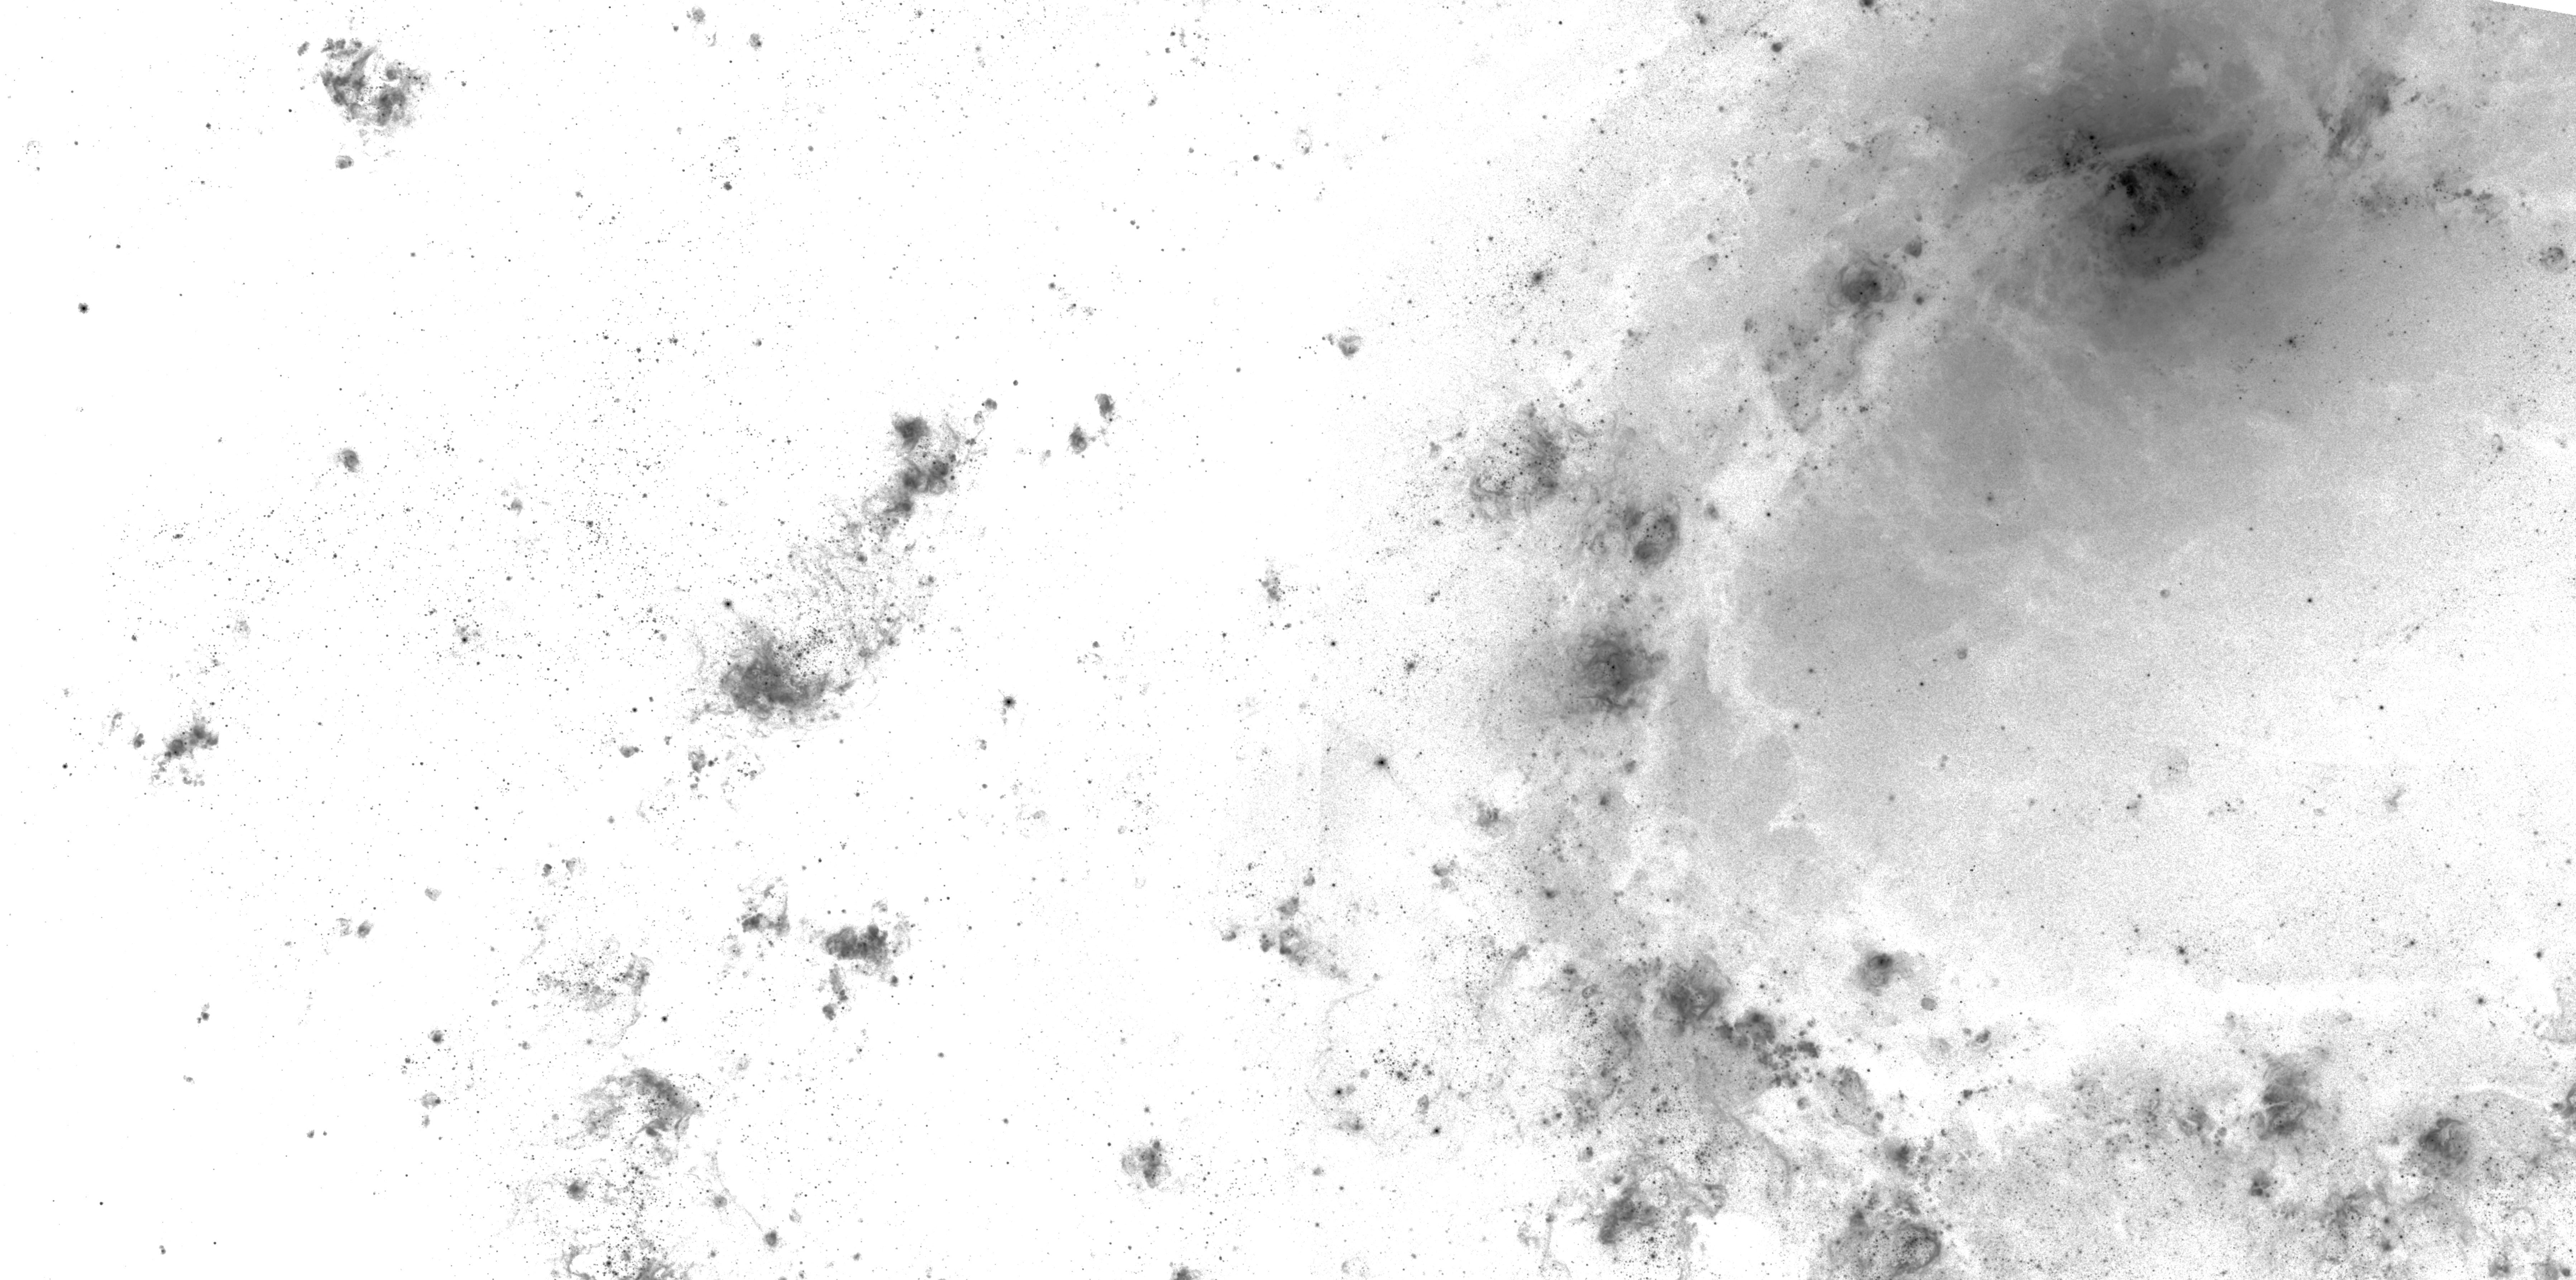
\includegraphics[width=0.77\textwidth]{ha-gray-conv-crp.jpg}
    \caption{Picture of the M83 galaxy, image taken from the WFC3 ERS M83 Data Products, http://archive.stsci.edu/prepds/wfc3ers/m83datalist.html}
    \label{fig:awesome_image}
\end{figure}

How can we learn something about this image, quantize, get useful information? In the next subsections I will explain the first ideas.

\subsection{Superpixel segmentation}
The main concept of this is to cut an image into bigger neighbourhood sections, so from an image that has $425x10^5$ pixels we can get maybe less than 500 superpixels, and then analyse separately those little sections and identify what kind of interstellar objects are they, look at image \ref{fig:super} it is a self-explanatory example of how a superpixel algorithm works.
\begin{figure}[h]
    \centering
    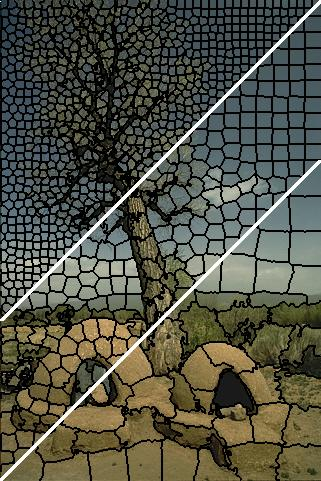
\includegraphics[width=0.37\textwidth]{combo.jpg}
    \caption{Example of a superpixel algorithm}
    \label{fig:super}
\end{figure}
There are many ways to do this and they vary according to color dimensions, methods and number of required superpixels and whether the algorithm is able to find borders and make pixel classifications.

\begin{remark}
	You can find some example test I tested with Matlab and with Python in this web page: \url{https://github.com/LaurethTeX/Clustering/blob/master/Methods.md}, also there is a huge amount of information on the internet about this but here are two pages you might find useful:
    \begin{itemize}
    	\item Superpixel: Empirical Studies and Applications \\ \url{http://ttic.uchicago.edu/~xren/research/superpixel/}
        \item Segmentation Algorithms in scikits-image \\ \url{http://peekaboo-vision.blogspot.ca/2012/09/segmentation-algorithms-in-scikits-image.html}
    \end{itemize}
    Also there is one article (from IEEE) I found about and might interest you, it's pure computer science,
    \begin{itemize}
    	\item Normalized Cuts and Image Segmentation \\ \url{http://www.cs.berkeley.edu/~malik/papers/SM-ncut.pdf}
    \end{itemize}
\end{remark}

\subsection{PCA}

Welcome to Astronomy where you will find more acronyms than words to mention something on articles, lots of fun!, well in this case PCA stands for Principal Component Analysis, the objective of this method is to reduce dimensionality, transform the data to another space where is can be manipulated and reduced, there are multiple examples of work that has been done in astronomy applying this technique.

Therefore, the idea of applying this method is that if we have multiple-wavelength images of the same target and transform them to PCA space then we will have less dimensionality and it will be easier to process all the data and fins valuable information.\footnote{Before I forget to mention, later I discovered that PCA is not commonly used for data mining preprocessing because it is hard to interpret the information in the output result. Imagine clusters of data on PCA space, how do you make sense to that?}

\begin{figure}[h]
    \centering
    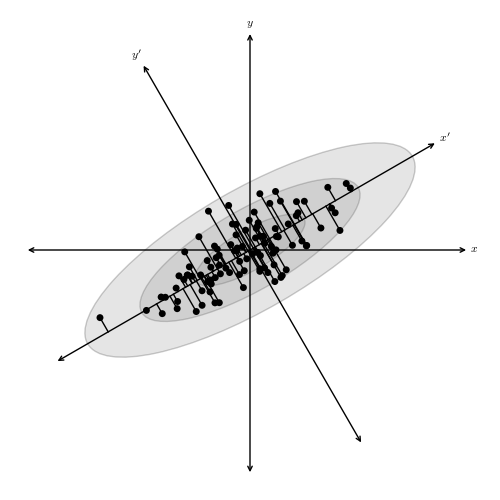
\includegraphics[width=0.37\textwidth]{fig_PCA.png}
    \caption{A distribution of points drawn from a bivariate Gaussian and centred on the origin of $x$ and $y$. PCA defines a rotation such that the new axes ($x’$ and $y’$) are aligned along the directions of maximal variance (the principal components) with zero covariance. This is equivalent to minimizing the square of the perpendicular distances between the points and the principal components}
    \label{fig:pca}
\end{figure}

\begin{remark}
	An example article, where they explain how to apply PCA on multi-wavelength images and also mentions the pros and cons of using it.
    \begin{itemize}
    	\item Preserving Structure in Multi-wavelength Images of Extended Objects\\ \url{http://arxiv.org/abs/1101.1679v1}
    \end{itemize}
    There's a whole section that talks about this subject with a machine learning approach as a preprocessing step in this nice book,
    \begin{itemize}
    	\item Ivezi{\'c}, \v Z. and Connolly, A.J.
         and Vanderplas, J.T. and Gray, A., \textit{Statistics, Data Mining and Machine Learning in Astronomy}, Princeton University Press, Princeton, NJ, 2014.
    \end{itemize}
\end{remark}

\section{Hypothesis}\index{Hypothesis}
Our data looks like the images on Fig.\ref{fig:cubes}, and it contains data from let's say a determined galaxy at different wavelengths, if we assume that the galaxy contains various regions that relate to interstellar objects that can tell, how stars are formed, where, how stars die, where was a star, and other mysteries, I guess we can assume that those certain regions can be identified because they share similar characteristics, the ideas is to find how a galaxy is made from, its contents, apply the concept of the superpixel idea in 3D superpixels. 
\begin{figure}[h]
	\centering
    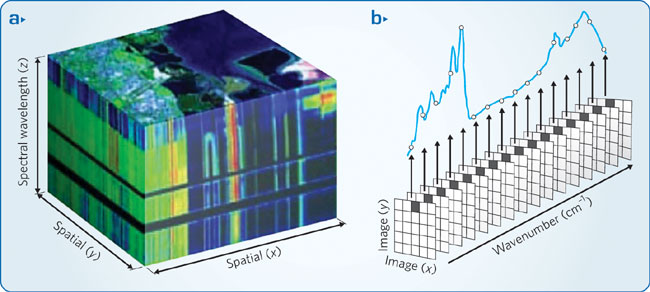
\includegraphics[width=0.57\textwidth]{nphoton.jpg}\hspace{1cm}
    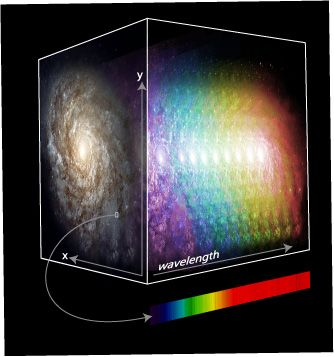
\includegraphics[width=0.27\textwidth]{data.jpg}
    \caption{Illustrations of how a data cube looks like.}
    \label{fig:cubes}
\end{figure}

Take the time to think about this, how the data looks like in 3D, how a star looks like in the data cube, imagine it, this is where ideas of how to tackle this problem come from.
\begin{figure}
	\centering
    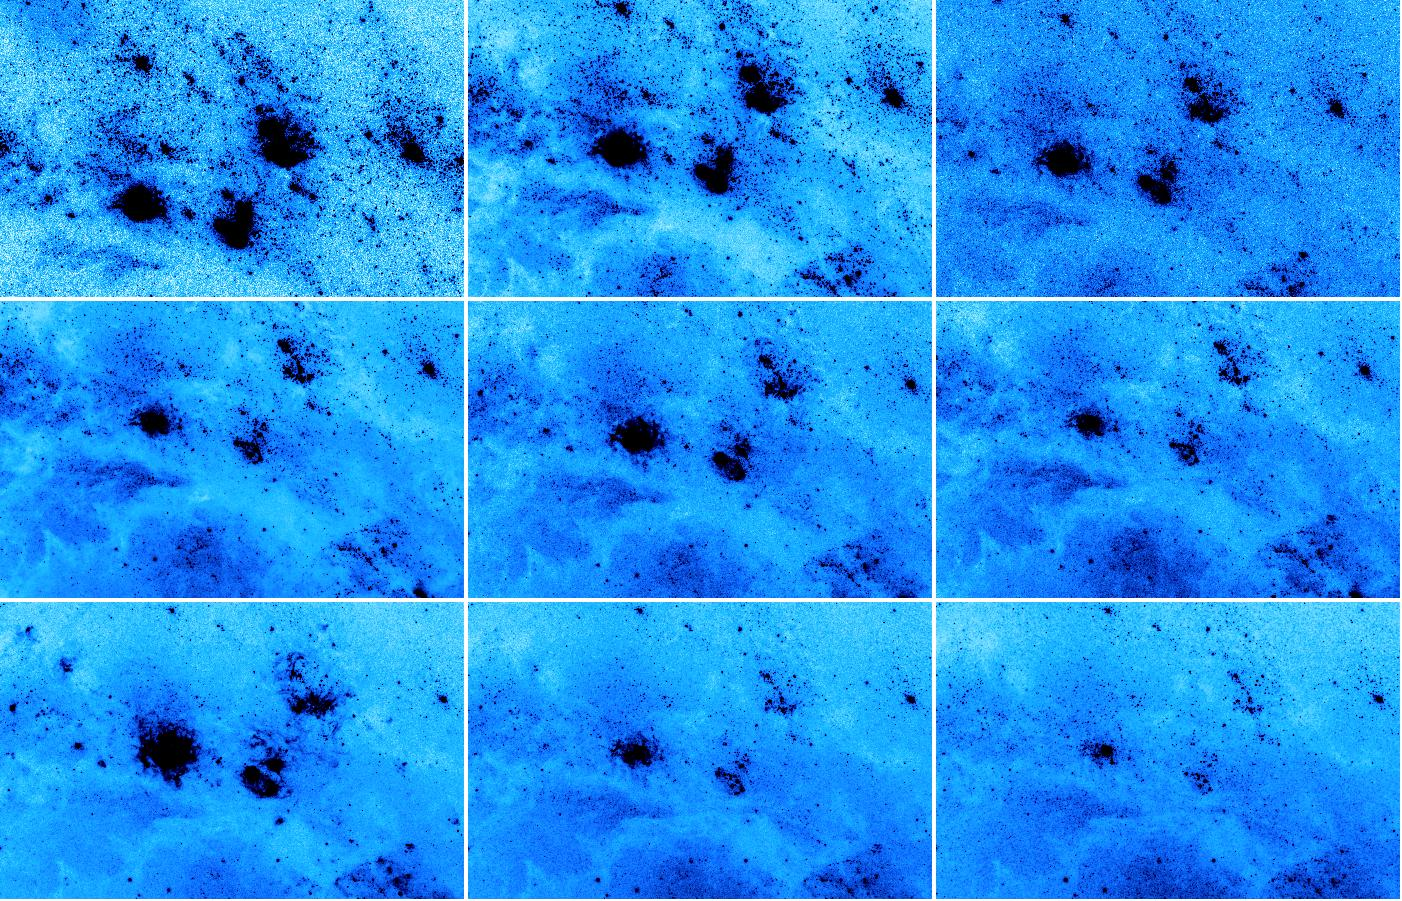
\includegraphics[width=0.87\textwidth]{nine.jpg}
    \caption{Example of how an object can look in 9 wavelengths}
    \label{fig:nine}
\end{figure}

\subsection{Topics you should review}\index{Related topics}
This will require a lot of work, but hey it will be worthy and fun!
\begin{itemize}
	\item Astroinformatics and computer science
    	\begin{itemize}
        	\item Data mining
            \item Machine Learning
            \item Big Data Analysis
            \item Neural Networks
            \item Visualization Resources
        \end{itemize}
    \item Statistics and Image Processing
    	\begin{itemize}
        	\item Probability Density Function
            \item Point Spread Function
            \item Full width at half maximum
            \item Convolution
        \end{itemize}
    \item Interstellar medium and star formation
    	\begin{itemize}
        	\item HII regions
            \item Planetary Nebulae
            \item Supernova Remnants
            \item Molecular Gas
            \item All kinds of Nebulae (e.g. dark, reflection)
            \item AGN's (Active Galactic Nucleus)
        \end{itemize}
    \item Astrophysics
    	\begin{itemize}
        	\item Units (light-years, parsecs)
            \item World coordinate system
        	\item Light
            \item Telescopes
            \item Stars and Stellar Evolution
            \item Distance, Brightness, Luminosity
            \item Galaxies
        \end{itemize}
\end{itemize}
The GitHub page will certainly help you to understand why you need to learn about that, and where to find articles, web pages and books.
\subsection{Downloading}
First, let's equip ourselves with the basic software you will need in order to start then you may probably find other cool programs and later you will install them. There is also the possibility that your assigned computer will have them installed already but here is a brief description of what you can do with them, most of them are easy to use.

\begin{description}
	\item[DS9:] It is a program that visualizes astronomy images in FITS format (don't worry if you recognize this format, it will be explained later), where you can easily manipulate them, read their headers, compare, look at regions, see their characteristics, make graphs, even videos. Well, depending on what you need to use later you will be finding all the functions, the best way is to click everywhere and find out what happens, also you can ask to your astronomy colleagues they will tell you all the perks, or if you like learning by yourself or you need something specific check the documentation web page. It is fairly easy to install, just follow the instructions.
    	\begin{description}
        	\item[Download: ]\url{http://ds9.si.edu/site/Download.html}
            \item[Documentation: ]\url{http://ds9.si.edu/site/Documentation.html}
        \end{description}
        The picture below shows (Fig.\ref{fig:screen}something cool you can do in DS9.
        \begin{figure}[h]
        	\centering
    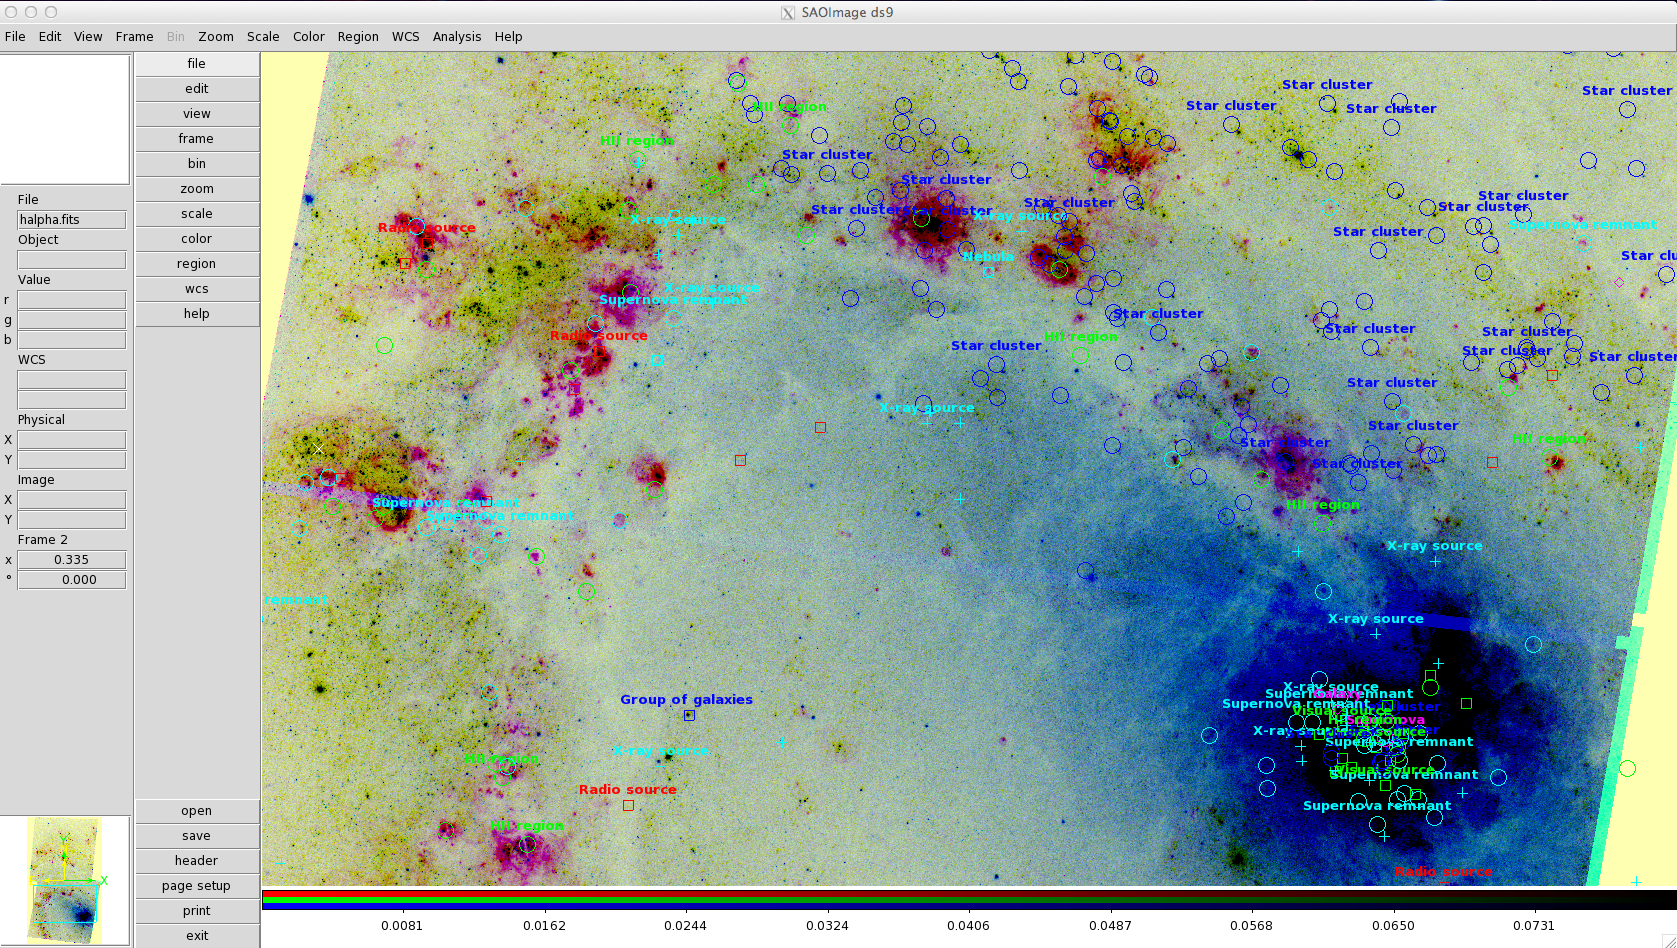
\includegraphics[width=0.87\textwidth]{Screenshot.png}
    \caption{This is an RGB picture made from 3 independent FITS files, with a z scale and a region file overlaid from NED database, if you would like to learn more about this, or reproduce it, it is all explained in this web page: \url{https://github.com/LaurethTeX/Clustering/blob/master/NEDtoREGION-FILE/KnownRegions.md}}
    \label{fig:screen}
        \end{figure}
        
    \item[Python and a user interface: ]The most \emph{limitless} and user friendly way to develop programs in Astronomy is using Python, there are many packages, modules, functions now available to help you in almost anything. Me, as an undergrad engineer I'm used to program on an user interface and not directly in a terminal. So, here I will explain you my own way of doing things.
    
    I make my programs on the Canopy editor, it shows when and where you have programming error and warnings, and the interface is easy to learn, now to run, I open a terminal, go to the directory where my program is, type \verb|ipython| wait and then type \verb|run| \verb|myProgram.py|, and wait for the result.
    
    Now there are a lot of fancier ways to work with \emph{Python}, you can program and test directly using \emph{IPython Notebook} on a web browser or you can just go for the terminal, use \emph{nano} or \emph{vi} or the text editor you like and then run it by typing \verb|python| \verb|myProgram.py|. At this point is up to you, but hey here are some links to start and the packages/modules you should install.
    
    \begin{description}
    	\item[Interfaces or Development environments]\hfill
        	\begin{itemize}
            	\item PyCharm, it a development environment, just like CodeBlocks or NetBeans \url{http://www.jetbrains.com/pycharm/}
                \item Spyder, actually this is the interface that comes with the Python distribution Anaconda, you will get the Python distribution and the interface. \url{https://store.continuum.io/cshop/anaconda/}
                \item Canopy, this is the one I mentioned before, it super easy to use and you can install packages with one click. \url{https://www.enthought.com/products/canopy/}
            \end{itemize}
        \item[Modules]\hfill
        \\
        In Python, modules are like the libraries in C, therefore, to use math, astronomy and computer science tools you need to install them. To learn whether you already have a module installed or not, type on \emph{iPython} \verb|import andreaModule|, if the output result is something like \verb|ImportError: No module named andreaModule|, you definitely don't have it installed. 
        
        The strategy here to install packages it fairly easy, find their website, go to the download section and follow the instructions, almost all the packages are available on the Python Packaging Index and may be installed by running:
        \begin{verbatim}
        	pip install pyfits
        \end{verbatim}
        To learn how to use them check the documentation page, user manuals or their API's, if you have experience on object oriented programming it will be like running a new bike and if you don't, don't worry too much, Python was designed to be easy to program, just learn the rules of the game.
        	\begin{itemize}
            	\item Astropy, this package is the \emph{must have} of every astronomer, contains tools to handle coordinate systems, units, convolution.. well is better if you take a look at the web page. \url{http://www.astropy.org/}
                \item Numpy, this package contains the math magic functions, linear algebra tools and the array management variables, make sure you learn all about \emph{Numpy arrays} you will work with them all the time. \url{http://www.numpy.org/}
                \item SciPy, well this package is the base of all scikit modules which contain the functions you will use in image processing and machine learning. \url{http://www.scipy.org/}
                	\begin{itemize}
                    	\item Scikit Image, contains image processing tools, it is the \emph{OpenCV} for \emph{Python} \url{http://scikit-image.org/}
                        \item Scikit Learn, contains data mining algorithms, pretty much contains everything that you will ever need. \url{http://scikit-learn.org/}
                    \end{itemize}
                \item Matplotlib, this package is probably one of the most powerful tools visualize data, you can draw almost anything you want and exactly how you want it. An example of that are the images of the AstroML book, you can access to the image library code and learn how they are made, this is the website \url{http://www.astroml.org/book_figures/index.html}.\footnote{Statistics, Data Mining, and Machine Learning in Astronomy book, it was mentioned before}. You can download the package here \url{http://matplotlib.org/}.
                \item PyFITS, in this package you will find tools to manipulate FITS files, create new ones, create image cubes, tables, and do all kinds of things with their headers. Certainly this package is more than useful. \url{http://www.stsci.edu/institute/software_hardware/pyfits}
            \end{itemize}
    \end{description}
    In the path of researching I'm certain you will find more and new packages and by them you will be prepared to install anything.
    \item[Montage: ]This is a toolkit for assembling astronomical images into mosaics, but it has more functions that you may need in the future to prepare your data before processing it. There are two ways of installing and I would say that is better to have them both. One is to install the toolkit and any time you need it, you run the commands on the terminal, the other one is to install a \emph{Python} module and use it just like any other module.
    To install montage for terminal, download the latest version in this website \url{http://montage.ipac.caltech.edu/docs/download.html}, \textbf{read the README file} or go to this website \url{http://montage.ipac.caltech.edu/docs/build.html} and follow the steps, now if you don't have any problem installing it, you can try testing it with an example program found on this website \url{http://montage.ipac.caltech.edu/docs/pleiades_tutorial.html}, in case you are having trouble and your computer is a MAC, instead of doing step five (\emph{If you want to be able to run the Montage executables from any directory}), try this:
    
    \begin{enumerate}
    	\item Open a file called \verb|.profile| located in your user folder. (e.g. \verb|/Users/Laureth|)
        	\begin{verbatim}
            	$ vi .profile
            \end{verbatim}
         \item Include in the file the following
           \begin{verbatim}
           	export PATH=/Applications/Montage_v3.3/bin:$PATH
           \end{verbatim}
           In this link (\url{https://github.com/LaurethTeX/Clustering/blob/master/Tools.md#the-profile-file}) you will find an example of how this file should look. After you modify it, make sure that you save it and type in \verb|/Users/Laureth|,
           \begin{verbatim}
           	$ source .profile
           \end{verbatim}
           Then try testing the \emph{Montage} commands, and I'm sure that it will magically work, just remember that any time you use any command, type \verb|source .profile|.\\
            
    \end{enumerate}
    
    
    
      Now the other way to install, implies only to install a \emph{Python} module but this module contains less functions that the terminal application, in any case check the website \url{http://www.astropy.org/montage-wrapper/}, there you will find all the documentation you may need and the instructions to install it (\emph{Spoilers} \verb|pip install montage-wrapper| ).\\
\end{description}

Any questions you may have and how to install, here is my GitHub page for software tools \url{https://github.com/LaurethTeX/Clustering/blob/master/Tools.md}
